% Options for packages loaded elsewhere
\PassOptionsToPackage{unicode}{hyperref}
\PassOptionsToPackage{hyphens}{url}
%
\documentclass[
]{book}
\usepackage{lmodern}
\usepackage{amsmath}
\usepackage{ifxetex,ifluatex}
\ifnum 0\ifxetex 1\fi\ifluatex 1\fi=0 % if pdftex
  \usepackage[T1]{fontenc}
  \usepackage[utf8]{inputenc}
  \usepackage{textcomp} % provide euro and other symbols
  \usepackage{amssymb}
\else % if luatex or xetex
  \usepackage{unicode-math}
  \defaultfontfeatures{Scale=MatchLowercase}
  \defaultfontfeatures[\rmfamily]{Ligatures=TeX,Scale=1}
\fi
% Use upquote if available, for straight quotes in verbatim environments
\IfFileExists{upquote.sty}{\usepackage{upquote}}{}
\IfFileExists{microtype.sty}{% use microtype if available
  \usepackage[]{microtype}
  \UseMicrotypeSet[protrusion]{basicmath} % disable protrusion for tt fonts
}{}
\makeatletter
\@ifundefined{KOMAClassName}{% if non-KOMA class
  \IfFileExists{parskip.sty}{%
    \usepackage{parskip}
  }{% else
    \setlength{\parindent}{0pt}
    \setlength{\parskip}{6pt plus 2pt minus 1pt}}
}{% if KOMA class
  \KOMAoptions{parskip=half}}
\makeatother
\usepackage{xcolor}
\IfFileExists{xurl.sty}{\usepackage{xurl}}{} % add URL line breaks if available
\IfFileExists{bookmark.sty}{\usepackage{bookmark}}{\usepackage{hyperref}}
\hypersetup{
  pdftitle={Aplicaciones de electrónica digital},
  pdfauthor={Josué Meneses Díaz},
  hidelinks,
  pdfcreator={LaTeX via pandoc}}
\urlstyle{same} % disable monospaced font for URLs
\usepackage{longtable,booktabs}
\usepackage{calc} % for calculating minipage widths
% Correct order of tables after \paragraph or \subparagraph
\usepackage{etoolbox}
\makeatletter
\patchcmd\longtable{\par}{\if@noskipsec\mbox{}\fi\par}{}{}
\makeatother
% Allow footnotes in longtable head/foot
\IfFileExists{footnotehyper.sty}{\usepackage{footnotehyper}}{\usepackage{footnote}}
\makesavenoteenv{longtable}
\usepackage{graphicx}
\makeatletter
\def\maxwidth{\ifdim\Gin@nat@width>\linewidth\linewidth\else\Gin@nat@width\fi}
\def\maxheight{\ifdim\Gin@nat@height>\textheight\textheight\else\Gin@nat@height\fi}
\makeatother
% Scale images if necessary, so that they will not overflow the page
% margins by default, and it is still possible to overwrite the defaults
% using explicit options in \includegraphics[width, height, ...]{}
\setkeys{Gin}{width=\maxwidth,height=\maxheight,keepaspectratio}
% Set default figure placement to htbp
\makeatletter
\def\fps@figure{htbp}
\makeatother
\setlength{\emergencystretch}{3em} % prevent overfull lines
\providecommand{\tightlist}{%
  \setlength{\itemsep}{0pt}\setlength{\parskip}{0pt}}
\setcounter{secnumdepth}{5}
\usepackage{booktabs}
\usepackage{booktabs}
\usepackage{longtable}
\usepackage{array}
\usepackage{multirow}
\usepackage{wrapfig}
\usepackage{float}
\usepackage{colortbl}
\usepackage{pdflscape}
\usepackage{tabu}
\usepackage{threeparttable}
\usepackage{threeparttablex}
\usepackage[normalem]{ulem}
\usepackage{makecell}
\usepackage{xcolor}
\ifluatex
  \usepackage{selnolig}  % disable illegal ligatures
\fi
\usepackage[]{natbib}
\bibliographystyle{apalike}

\title{Aplicaciones de electrónica digital}
\author{Josué Meneses Díaz}
\date{2021-07-26}

\begin{document}
\maketitle

{
\setcounter{tocdepth}{1}
\tableofcontents
}
\listoftables
\listoffigures
\hypertarget{introducciuxf3n}{%
\chapter{Introducción}\label{introducciuxf3n}}

Los siguientes apuntes muestran diversas aplicaciones de circuitos digitales como complemento al curso ``electrónica digital y microcontroladores'' para la carrera de Ingeniería en Física.

\begin{itemize}
\tightlist
\item
  Propósito del circuito.
\item
  Método de resolución ha utilizar.
\item
  Esquema del circuito
\end{itemize}

\hypertarget{intro}{%
\chapter{Lógica combinacional}\label{intro}}

En esta sección se presenta una colección de circuitos lógicos combinacionales aplicando diferentes métodos de análisis.

Para cada uno de las aplicaciones mostradas se presenta:

\begin{itemize}
\tightlist
\item
  Propósito del circuito.
\item
  Método de resolución ha utilizar.
\item
  Esquema del circuito
\end{itemize}

Los programas utilizados para el desarrollo de los circuitos han sido:

\begin{itemize}
\tightlist
\item
  \textbf{Losigim-evolution} para las pruebas y diseño de los circuitos combinacionales.
\item
  \textbf{xcircuit} para la creación de los diagramas finales.
\end{itemize}

\hypertarget{medio-sumador}{%
\section{Medio Sumador}\label{medio-sumador}}

Se conoce como medio sumador al circuito combinacional que permite realizar la operación se suma aritmética entre dos números binarios enteros \emph{considerando solamente un acarreo de salida}.

\hypertarget{entradas-y-salidas}{%
\subsection{Entradas y salidas}\label{entradas-y-salidas}}

El circuito posee dos posibles entradas:

\begin{itemize}
\tightlist
\item
  \(A\)
\item
  \(B\)
\end{itemize}

Recordando que el número máximo de bit en la salida de un sumador es igual a \[
  \max\{nbit(A), nbit(B)\}+1
\] Para este caso, el máximo número de bits entre \(A\) y \(B\) será 1 por lo que en la salida tendremos, a lo más, dos bits:

\begin{itemize}
\tightlist
\item
  El resultado de la suma mediante la función \(S\)
\item
  El acarreo de salida mediante la función \(A_{out}\)
\end{itemize}

\hypertarget{tabla-de-verdad}{%
\subsection{Tabla de verdad}\label{tabla-de-verdad}}

\begin{longtable}[]{@{}cccc@{}}
\caption{Tabla de verdad para el circuito de medio sumador binario.}\tabularnewline
\toprule
A & B & S & \(A_{out}\)\tabularnewline
\midrule
\endfirsthead
\toprule
A & B & S & \(A_{out}\)\tabularnewline
\midrule
\endhead
0 & 0 & 0 & 0\tabularnewline
0 & 1 & 1 & 0\tabularnewline
1 & 0 & 1 & 0\tabularnewline
1 & 1 & 0 & 1\tabularnewline
\bottomrule
\end{longtable}

\hypertarget{funciuxf3n-booleana-mediante-minituxe9rminos-e-implementaciuxf3n}{%
\subsection{Función booleana mediante minitérminos e implementación}\label{funciuxf3n-booleana-mediante-minituxe9rminos-e-implementaciuxf3n}}

\begin{aligned}
S(A, B) &=& \sum m(1,2)\\
        &=& m_1+m_2\\
        &=& \bar{A} B + A \bar{B}\\
\end{aligned}

Esta última es equivalente a la puerta lógica XOR (Puerta or exclusiva)

\[
S(A, B) = A\oplus B
\]

La salida \(A_{out\) para el acarreo de salida será

\begin{aligned}
   A_{out} &=& AB\\
\end{aligned}

\hypertarget{funciuxf3n-booleana-mediante-maxituxe9rminos-e-implementaciuxf3n}{%
\subsection{Función booleana mediante maxitérminos e implementación}\label{funciuxf3n-booleana-mediante-maxituxe9rminos-e-implementaciuxf3n}}

\begin{aligned}
S(A, B) &=& \prod M(0,3)\\
        &=& M_0\cdot M_3\\
        &=& (A+B)⋅(\bar{A}+\bar{B})\\
\end{aligned}

La salida \(A_{out}\) para el acarreo de salida será

\begin{aligned}
   A_{out} &=& \prod M(0,1,2)\\
           &=& M_1\cdot M_2 \cdot M_3\\
           &=& (A+B)(A+\bar{B})(\bar{A}+B)\\
           &=& (A+B)(A\bar{A}+AB+\bar{A}\bar{B}+B\bar{B})\\ 
           &=& (A+B)(AB+\bar{A}\bar{B})\\ 
           &=& AAB+A\bar{A}\bar{B}+ABB+\bar{A}B\bar{B}\\ 
           &=& AB+AB\\ 
           &=& AB\\ 
\end{aligned}

\hypertarget{funciuxf3n-booleana-mediante-k-map}{%
\subsection{Función booleana mediante k-map}\label{funciuxf3n-booleana-mediante-k-map}}

\begin{figure}

{\centering 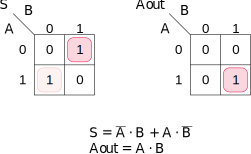
\includegraphics[width=0.5\linewidth]{./images/kmap medio sumador} 

}

\caption{Mapas de Karnaugh para el circuto de medio sumador binario}\label{fig:unnamed-chunk-1}
\end{figure}

TODO:

\begin{itemize}
\tightlist
\item
  Circuito equivalentes
\end{itemize}

\hypertarget{sumador-completo}{%
\section{Sumador completo}\label{sumador-completo}}

A diferencia el circuito de medio sumador, este circuito considera un acarreo de entrada junto con los bits de los números \(A\) y \(B\), permitiendo extender el uso de este diseño a sumadores de n-bits.

\hypertarget{medio-restador-binario}{%
\section{Medio Restador Binario}\label{medio-restador-binario}}

Definimos el caso de un restador de 1 bit utilizando el concepto de \emph{prestamo}

\begin{verbatim}
## Warning: package 'kableExtra' was built under R version 4.0.5
\end{verbatim}

\begin{table}
\centering
\begin{tabular}{r|r|r|r}
\hline
\multicolumn{2}{c|}{Entrada} & \multicolumn{2}{c}{Salida} \\
\cline{1-2} \cline{3-4}
A & B & Prestamo & R\\
\hline
0 & 0 & 0 & 0\\
\hline
0 & 1 & 1 & 1\\
\hline
1 & 0 & 0 & 1\\
\hline
1 & 1 & 0 & 0\\
\hline
\end{tabular}
\end{table}

\hypertarget{funciuxf3n-booleana-mediante-minituxe9rminos-e-implementaciuxf3n-1}{%
\subsection{Función booleana mediante minitérminos e implementación}\label{funciuxf3n-booleana-mediante-minituxe9rminos-e-implementaciuxf3n-1}}

\begin{aligned}
S(A, B) &=& \sum m(1,2)\\
        &=& m_1+ m_1\\
        &=& \bar{A}B + A\bar{B}\\
        &=& A \oplus B\\
\end{aligned}

\begin{aligned}
P(A, B) &=& \sum m(1)\\
        &=& m_1\\
        &=& \bar{A}B\\
\end{aligned}

Luego la implementación mediante puertas lógicas es tan simple como:

\begin{figure}

{\centering \includegraphics[width=0.6\linewidth]{./images/circuito restador simple} 

}

\caption{Circuito equivalente para restador binario utilizando función de prestamo}\label{fig:unnamed-chunk-3}
\end{figure}

\hypertarget{restador-completo}{%
\section{Restador completo}\label{restador-completo}}

Al igual que el sumador completo, el restador completo considera un 3er bit de entrada (prestamo de entrada) que permite extender este circuito hasta n-conexiones.

La tabla de verdad para este circuito por lo tanto considera tres entradas:

\begin{itemize}
\tightlist
\item
  \(A\)
\item
  \(B\)
\item
  \(P_{in}\)
\end{itemize}

Y dos salidas

\begin{itemize}
\tightlist
\item
  \(R\)
\item
  \(P_{out}\)
\end{itemize}

\begin{table}
\centering
\begin{tabular}{r|r|r|r|r}
\hline
\multicolumn{3}{c|}{Entrada} & \multicolumn{2}{c}{Salida} \\
\cline{1-3} \cline{4-5}
A & B & Pin & Pout & R\\
\hline
0 & 0 & 0 & 0 & 0\\
\hline
0 & 0 & 1 & 1 & 1\\
\hline
0 & 1 & 0 & 1 & 1\\
\hline
0 & 1 & 1 & 1 & 0\\
\hline
1 & 0 & 0 & 0 & 1\\
\hline
1 & 0 & 1 & 0 & 0\\
\hline
1 & 1 & 0 & 0 & 0\\
\hline
1 & 1 & 1 & 1 & 1\\
\hline
\end{tabular}
\end{table}

\hypertarget{circuito}{%
\subsection{Circuito}\label{circuito}}

\begin{figure}

{\centering 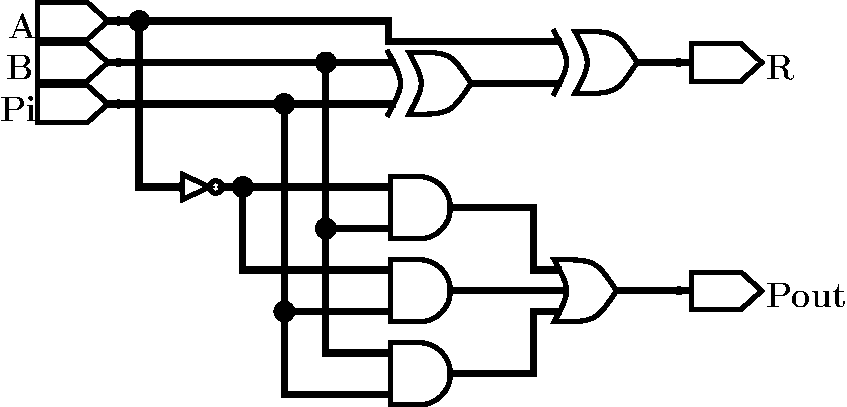
\includegraphics[width=0.6\linewidth]{./images/circRestadorCompleto} 

}

\caption{Circuito del restador completo utilizando puertas xor}\label{fig:unnamed-chunk-5}
\end{figure}

\hypertarget{conexiuxf3n-en-cascada}{%
\subsection{Conexión en cascada}\label{conexiuxf3n-en-cascada}}

Utilizando el circuito de restador completo de 1 bits podemos extender el circuito a un restador de n-bits conectando en cascada n circuitos restadores de 1 bits. Por ejemplo, utilizando 4 circuitos restadores completos de 1 bits conectando las salidas de prestamo a las entradas de préstamo del siguiente circuito como:

\begin{figure}

{\centering 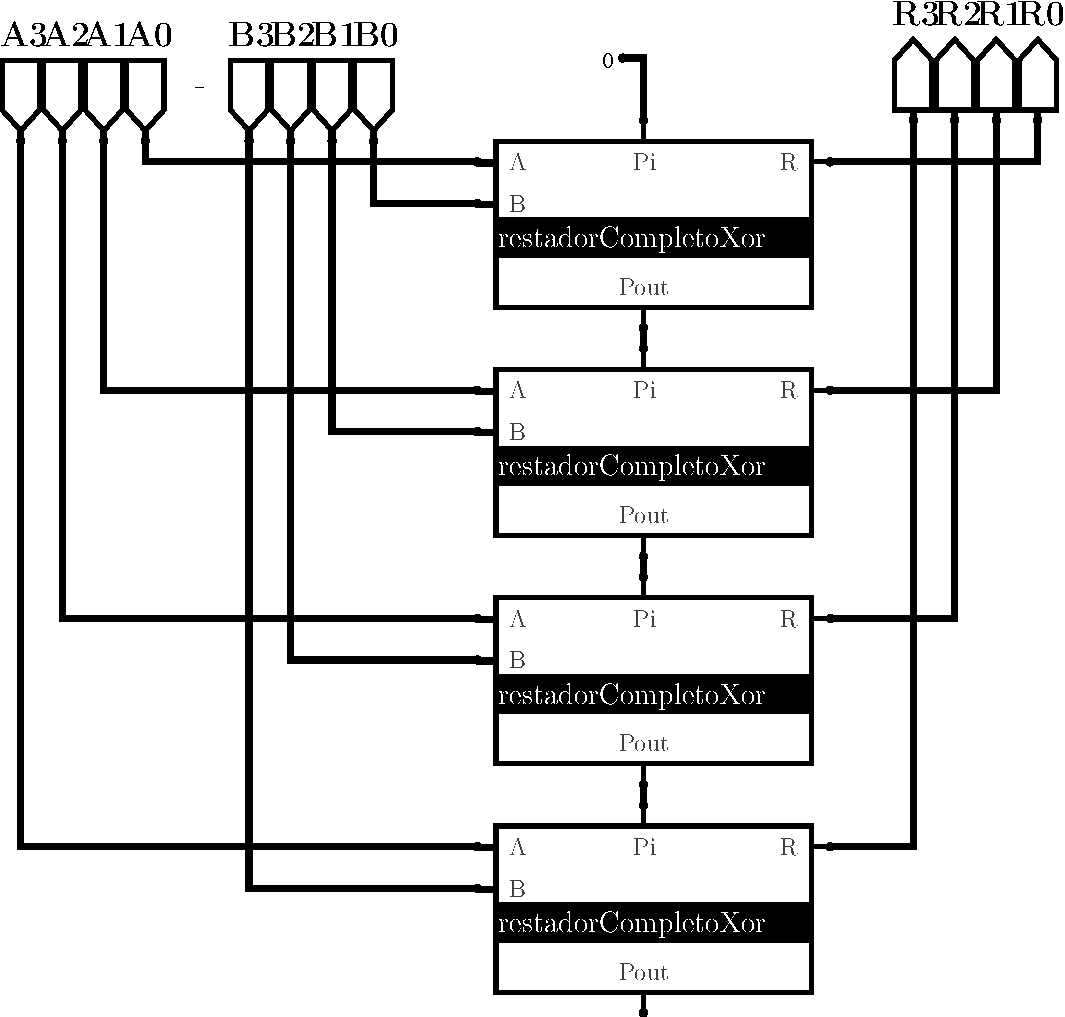
\includegraphics[width=0.6\linewidth]{./images/circRestador4bits} 

}

\caption{Circuito restador de 4 bits utilizando 4 circuitos restadores completos de 1 bits en conexion cascada.}\label{fig:unnamed-chunk-6}
\end{figure}

\hypertarget{multiplexor-mux}{%
\section{Multiplexor (MUX)}\label{multiplexor-mux}}

El circuito Multiplexor tiene como finalidad conectar \textbf{una de las multiples entradas} del circuito a la salida \(Y\), en otras palabras, los Multiplexores son switches digitales. La elección de que linea de entrada será conectada con la salida del circuito es realizada mediante unas entradas llamadas ``lineas de selección''. Normalmente, los MUX poseen \(2^n\) lineas de entrada y \(n\) lineas de selección. Las entradas de selección utilizan la numeración binaria para seleccionar la entrada a conectar.

\hypertarget{implementaciuxf3n-de-entrada-habilitante}{%
\subsection{Implementación de entrada habilitante}\label{implementaciuxf3n-de-entrada-habilitante}}

\hypertarget{methods}{%
\chapter{Methods}\label{methods}}

We describe our methods in this chapter.

\hypertarget{applications}{%
\chapter{Applications}\label{applications}}

Some \emph{significant} applications are demonstrated in this chapter.

\hypertarget{example-one}{%
\section{Example one}\label{example-one}}

\hypertarget{example-two}{%
\section{Example two}\label{example-two}}

\hypertarget{final-words}{%
\chapter{Final Words}\label{final-words}}

We have finished a nice book.

  \bibliography{book.bib,packages.bib}

\end{document}
